\documentclass[11pt,fleqn]{article}

\textheight=23.3cm
\textwidth=16.5cm
\topmargin=-15mm
\oddsidemargin=0cm

\usepackage{enumerate}
\usepackage{amsmath}
\usepackage{amssymb}
\usepackage{bbm}
\usepackage{graphicx}
\usepackage{wrapfig}
\usepackage{pdflscape}
\usepackage[sidewaysfigure]{rotating}
\usepackage{natbib}
\usepackage{multirow}
\newcommand{\tb}{\hspace*{3mm}}
\bibpunct{(}{)}{;}{a}{,}{,}
\parskip=3mm
\parindent=5mm
\baselineskip=17pt

\usepackage{amsthm}
\newtheorem{assumption}{Assumption}
\newtheorem{definition}{Definition}
\newtheorem{proposition}{Proposition}

\DeclareMathOperator*{\argmax}{arg\,max}

\usepackage{hyperref}
\hypersetup{
  pdftitle={Huggett \& Ventura (1999) - On the Distributional Effects of Social Security Reform},
  pdfauthor={Robert Kirkby},
  colorlinks=true,
  linkcolor=black,
  citecolor=black,
  urlcolor=blue,
  breaklinks=true
}

\begin{document}

\title{Replication of Huggett \& Ventura (1999)\\
\large ``On the Distributional Effects of Social Security Reform''}
\author{Robert Kirkby}
\date{\today}
\maketitle

\section{Introduction}\label{sec:intro}

Huggett \& Ventura (1999, hereafter HV1999) ask who wins and who loses from replacing the
U.S.\ social security system with the two-tier scheme proposed by the Bipartisan Commission
on Entitlement and Tax Reform (the ``Boskin proposal''): a defined-contribution annuity
proportional to the social security taxes an agent has paid, together with a floor benefit
$\underline{b}$ paid to any retiree whose annuity falls below it. The paper's central finding
is distributional rather than aggregate. Aggregates barely move across the reforms, but the
welfare consequences are sharply graded by ability, and at positive floor levels they are
\emph{U-shaped}: low- and high-ability agents gain while agents of median ability lose.

This document replicates the paper with the VFI Toolkit. Everything in HV1999 that reports
model output is covered: Tables III--VI and Figures 1--6, under both of the paper's two wage
specifications. Section~\ref{sec:model} states the model, Section~\ref{sec:calib} the
calibration and the data inputs, and Section~\ref{sec:ge} the equilibrium conditions --- in
particular how the floor benefit is financed, which the paper specifies in two places that
have to be read together. Section~\ref{sec:results} presents the results and
Section~\ref{sec:discrep} the differences from the paper that remain. Everything specific to
the numerical implementation is gathered in Appendix~\ref{sec:computational}.

The replication is close on aggregates and on the qualitative distributional findings. $K/Y$
is within $0.05$ of HV1999 in every row of Tables III and IV, the interest rate within
$0.2$ percentage points, and the income Gini matches to the two digits the paper reports. The
U-shape in the compensating variations replicates, as does the paper's argument about why
retaining the medical transfer mitigates the welfare losses. Two quantities are off: the
aggregate labour input $L$ and the fraction of time worked each sit about $8$ and $11$ percent
above the paper in \emph{both} specifications and at every floor level, and the welfare
aggregates of Tables V and VI run roughly twice as negative as HV1999's.

\section{Model}\label{sec:model}

Agents live at most $J=81$ periods, entering at real-life age 20 and facing age-dependent
survival probabilities $s_j$. There is no annuity market, so the assets of the deceased are
accidental bequests. All variables below are detrended by the technology level, which is
where the $(1+g)$ factors come from. Parameter values are collected in Table~\ref{tab:params};
all are HV1999's, taken from the paper's Table I.

\begin{table}[htp]
\begin{center}
\begin{tabular}{llr}
\hline
Parameter & Description & Value \\
\hline
$J$        & Maximum lifespan (periods)            & 81 \\
$J_r$      & Retirement age (period)               & 46 \\
$\beta$    & Discount factor                       & 1.011 \\
$\sigma$   & Curvature of the utility aggregator   & 2.0 \\
$\nu$      & Consumption share in the aggregator   & 0.33 \\
$\alpha$   & Capital share                         & 0.36 \\
$\delta$   & Depreciation rate                     & 0.06 \\
$A$        & Total factor productivity             & 0.895944 \\
$n$        & Population growth rate                & 0.012 \\
$g$        & Technological growth rate             & 0.021 \\
$G/Y$      & Government consumption share          & 0.195 \\
$b/Y$      & Common medical/hospital transfer      & 0.1242 \\
\hline
\end{tabular}
\end{center}
\caption{Parameter values, all from Huggett \& Ventura (1999). The wage-process parameters
are specification-specific and are given in Section~\ref{sec:wage}.}
\label{tab:params}
\end{table}

An agent of age $j$ holds assets $a$, average past earnings $\bar{e}$ and productivity shock
$z$, and chooses hours $l\in[0,1)$ and next-period assets $a'$. Writing the problem
recursively, with $x=(a,\bar{e},z)$,
\begin{equation*}
 V_j(a,\bar{e},z) = \max_{l\in[0,1),\;a'\ge 0}
   \left\{\; \frac{\big(c^{\nu}(1-l)^{1-\nu}\big)^{1-\sigma}}{1-\sigma}
   \;+\; \beta\, s_j\, E\big[\,V_{j+1}(a',\bar{e}',z') \,\big|\, z\,\big] \;\right\}
\end{equation*}
subject to the budget constraint
\begin{equation*}
 c + (1+g)a' = a\big(1+r(1-\tau)\big) + (1-\tau-\theta_j)\,e(z,j)\,w\,l + b(x,j),
\end{equation*}
the law of motion for $\bar{e}$ given below, and the terminal condition $V_{J+1}\equiv 0$,
where $\theta_j=\theta$ while working and $0$ in retirement, $e(z,j)=\exp(z)\kappa_j$ is the
agent's labour endowment in efficiency units, and $b(x,j)$ is the social security benefit.
Retirement is mandatory at $J_r$. Production is Cobb--Douglas and government consumption is
a fixed share of output.

Average past earnings evolve as HV1999 equation (7), which is
\begin{equation*}
 \bar{e}' = \frac{\bar{e}\,(j-1) + \min\{\,e(z,j)\,l,\; e_{\max}\,\}}{j}
 \qquad (j<J_r), \qquad \bar{e}'=\bar{e} \quad (j\ge J_r),
\end{equation*}
where $e_{\max}$ is the cap on creditable earnings. Writing the state instead in units of mean
working-age earnings, so that the bend points and the cap sit at fixed grid values regardless
of the equilibrium wage, this becomes
\begin{equation*}
 \bar{e}' = \frac{\bar{e}\,(j-1) + \min\!\big(e(z,j)\,l/\bar{y}^{\,\text{mean}},\,2.47\big)}{j}
 \qquad (j<J_r), \qquad \bar{e}'=\bar{e} \quad (j\ge J_r).
\end{equation*}
Here $\bar{y}^{\,\text{mean}}$ is average earnings per working-age person measured in
efficiency units, $E\big[\exp(z)\,\kappa_j\,l \mid j<J_r\big]$. It is distinct from the
age profile $\kappa_j$: it depends on the equilibrium allocation, through hours and the
distribution of $z$, and so is carried as an equilibrium unknown (Section~\ref{sec:ge}). The
cap of $2.47$ and the bend points at $0.20$ and $1.24$ are then fixed numbers on the
$\bar{e}$ grid, which is the point of writing the state this way.

Under the Boskin proposal $\bar{e}$ is replaced by $a_2$, the accumulated value of social
security taxes paid, which follows HV1999 equation (10),
\begin{equation*}
 (1+g)\,a_2' = \big(a_2 + \theta\, e(z,j)\, w\, l\big)(1+r) \qquad (j<J_r).
\end{equation*}
\subsection*{Benefits}

Under the U.S.\ system (HV1999 equation 15) benefits are zero before $J_r$ and thereafter
\begin{equation*}
 b(x,j) = b + \frac{w\,\bar{y}^{\,\text{mean}}\,\mathrm{PIA}(\bar{e})}{(1+g)^{j-J_r}},
\end{equation*}
where $b$ is a common medical/hospital transfer calibrated to $0.1242\,Y$ and
$\mathrm{PIA}$ is the 1990--94 U.S.\ primary insurance amount schedule: $90\%$ of the first
$0.20$, $32\%$ to the second bend point at $1.24$, and $15\%$ above, in multiples of average
earnings, with creditable earnings capped at $2.47$. This schedule is Figure~\ref{fig:fig2}.

Under the Boskin proposal (equation 16) benefits are
$b(x,j)=\max\{\underline{b},\,C a_2/(1+g)^{j-J_r}\}$ for $j\ge J_r$, where $C$ is a
proportionality factor determined in equilibrium and $\underline{b}$ is the floor, set to
$0$, $0.15$, $0.25$ or $0.35$ times output per person. The payroll tax rate $\theta$ and
government consumption are held at their U.S.-system values throughout, as HV1999 p.514
requires.

Section~\ref{sec:medical} describes the third system the paper considers, in which the
medical transfer is retained alongside the Boskin annuity.

\section{Calibration and data inputs}\label{sec:calib}

\subsection*{The age-efficiency profile}

$\kappa_j$, the age-efficiency profile, is taken from Hansen (1993). HV1999 footnote 16: ``Hansen estimates median wage
rates in cross-sectional data for males in different age groups. We use his values for the
center of the age group and linearly interpolate to get the remaining values. We set the
labor endowment in efficiency units of agents at a real-life age of 75 to zero.'' We follow
this exactly, using Hansen's Table II male weights at the age-group centres
$17.5, 22, 29.5, 39.5, 49.5, 59.5$ and running the profile linearly to zero at 75. The
resulting profile is Figure~\ref{fig:fig1}, plotted with Hansen's tabulated values as markers.

\subsection*{Survival}

Mortality is the U.S.\ male life table. The published table is given at five-year exact ages,
so single-year values are obtained by interpolating $\log q_x$ rather than $q_x$ --- mortality
is approximately Gompertz, i.e.\ log-linear in age, so linear interpolation of the level
systematically understates mortality between knots. Survival at the terminal age is set to
zero so that the cohort is exhausted at 100.

\subsection*{The two wage specifications}\label{sec:wage}

HV1999 considers two processes for log productivity, both with the dispersion parameter chosen
so that the wage Gini for agents under 65 equals $0.35$.

\emph{No idiosyncratic shocks.} $(\gamma,\sigma_\epsilon^2)=(1,0)$ and
$\sigma_{y_1}^2=0.376$: ability is drawn at birth and perfectly preserved. This is a
\emph{permanent type} in the toolkit, not an exogenous state, and is implemented as 21
permanent types with masses from the binned normal.

\emph{Idiosyncratic shocks.} $\sigma_{y_1}^2=0.27$ with an AR(1),
$z' = \gamma z + \epsilon$, $\epsilon\sim N(0,\sigma_\epsilon^2)$. HV1999 fix
$\sigma_\epsilon^2=0.015$ and $\gamma=0.985$, chosen by the indirect-inference step described
on p.512. Here $z$ is a genuine exogenous state, and because $\bar{e}'$ and $a_2'$ depend on
it the model uses \texttt{experienceassetz}.

The discretization follows footnote 17 exactly: ``The shock $z$ in each model takes on 21
evenly spaced values between $-4\sigma_{y_1}$ and $4\sigma_{y_1}$. Transition probabilities
are calculated by integrating the area under the normal distribution conditional on the value
of $z$.'' We use 21 points on that interval with transitions obtained by integrating the
normal between grid midpoints, open-ended at both ends. Section~\ref{sec:discrep} notes that
this grid is coarse relative to the innovation standard deviation and that refining it moves
the wage Gini; we keep 21 points because that is the paper's own choice.

\section{Equilibrium and the financing of the floor}\label{sec:ge}

The stationary equilibrium conditions are: factor prices equal marginal products, the government budget balances, social security balances, and accidental bequests
are absorbed by the government. Under the U.S.\ system the unknowns are
$r$, $w$, $\tau$, $\theta$, $b$ and the normalisation $\bar{y}^{\,\text{mean}}$, with $\theta$
set by social security balance and $b=0.1242\,Y$.

The Boskin stage needs more care, because HV1999 specifies the financing of the floor in two
separate places that must be read together. On p.514 the paper says ``the proportionality
factor $C$ is then set so that benefit payments to current retirees equal current social
security tax payments (condition 6 in the definition of equilibrium)''. Taken literally and
applied to \emph{total} benefits, this would pin
$\sum \max\{\underline{b},Ca_2/(1+g)^{j-J_r}\} = \theta w L$, which drives $C$ towards zero as
the floor rises and leaves no residual to finance. But footnote 23 states that ``transfers
needed to finance $\underline{b}=0.35Y$ are on the order of 1.3--1.4\% of GDP in the no
idiosyncratic case. This results in income tax rates going from 18.7\% in the zero floor
situation to 22.3\% for $\underline{b}=0.35Y$.'' Those two statements are consistent only if
the payroll tax finances the \emph{annuity} and the floor top-up is a transfer out of general
revenue. We therefore impose
\begin{align*}
 \theta\, w\, L &= \textstyle\sum_{j\ge J_r} C a_2/(1+g)^{j-J_r},\\
 \tau(rK+wL) + \text{AccBeq} &= \tfrac{G}{Y}\,Y + \mathcal{T},\\
 \mathcal{T} &\equiv \textstyle\sum_{j\ge J_r}
   \Big[\max\big\{\underline{b},\,Ca_2/(1+g)^{j-J_r}\big\} - Ca_2/(1+g)^{j-J_r}\Big].
\end{align*}
The first condition makes the annuity self-financing on a pay-as-you-go basis, which is the
paper's ``the financing of benefits is always on a pay-as-you-go basis'' (p.515); the second
is the government budget. The residual $\mathcal{T}$ --- the sum of
$\max\{0,\underline{b}-\text{annuity}\}$ over retirees --- is
the transfer footnote 23 refers to. At $\underline{b}=0$ the bracket is identically zero and
the system collapses to the zero-floor case, which is a useful internal check: the
$\underline{b}=0$ equilibrium computed under this formulation reproduces the one computed
before it was introduced to every printed digit.

The reading is confirmed quantitatively. Footnote 23 is a statement about the
no-idiosyncratic economy, so it is directly comparable with Table III: we obtain an income
tax rate of \textbf{18.7\%} at a zero floor --- exactly the paper's figure --- rising to
$21.4\%$ at $\underline{b}=0.35Y$ against the paper's $22.3\%$, with a floor transfer of
$1.82\%$ of GDP against the paper's $1.3$--$1.4\%$.

The floor itself is a multiple of output per person and output is endogenous, so
$\underline{b}$ is carried as an equilibrium unknown with the condition
$\underline{b}=\text{frac}\times Y$, exactly as $b=0.1242\,Y$ is handled in the U.S.\ stage.

\subsection*{The Boskin proposal with medical benefits retained}\label{sec:medical}

HV1999 Section 4.2 observes that under the plain Boskin proposal median-ability agents lose
the common medical transfer as well as the redistribution built into the concave PIA formula,
and asks what happens if only the old-age component is reformed. The resulting third system is
specified in footnote 29: the payroll tax splits as $\theta=\theta_1+\theta_2$, where
$\theta_1$ is the rate that financed the common transfer in the U.S.\ economy and is held
fixed, $\theta_2$ becomes the rate at which earnings accumulate into $a_2$, and benefits at
retirement are $\max\{\underline{b},\, b + b(a_2,j)\}$. We recover
$\theta_1 = b\,\mu_{\text{ret}}/(wL)$ from the U.S.\ equilibrium, where $\mu_{\text{ret}}$ is
the mass of retirees, and accumulate $a_2$ at $\theta_2=\theta-\theta_1$. Agents continue to
pay the full $\theta$; the split governs only what each part finances.

One ambiguity should be recorded. Footnote 29's $\max\{\underline{b},\,b+b(a_2,j)\}$ is
implemented here with the floor applying to the \emph{total} retirement income from the
system. The alternative reading, $b+\max\{\underline{b},b(a_2,j)\}$, would apply the floor to
the annuity alone and would make the floor bind for more retirees at a given
$\underline{b}$.

\subsection*{Compensating variations}

The welfare measure is the usual consumption-equivalent variation for a newborn of each
ability level. Because period utility is $\big(c^{\nu}(1-l)^{1-\nu}\big)^{1-\sigma}/(1-\sigma)$,
scaling an agent's consumption possibilities by $(1+x)$ at every date and state leaves optimal
hours unchanged and scales lifetime utility by $(1+x)^{\nu(1-\sigma)}$. Hence
\begin{equation*}
 \text{CEV}_i = \left(\frac{V^{\text{Boskin}}_i(0,0,1)}{V^{\text{US}}_i(0,0,1)}\right)^{\frac{1}{\nu(1-\sigma)}} - 1,
\end{equation*}
evaluated at the newborn state (zero assets, zero $\bar{e}$ or $a_2$, age 1). This is exact for
this utility function, so no re-solve or policy-evaluation step is required. The aggregate
measures of Tables V and VI apply the same transformation to the ability-weighted expected
newborn value, i.e.\ the welfare of an agent behind the veil of ignorance about ability.

\section{Results}\label{sec:results}

\subsection*{Aggregates: Tables III and IV}

Tables~\ref{tab:table3} and~\ref{tab:table4} report the general features of the model
economies under the two wage specifications. $K/Y$ is within $0.05$ of HV1999 in every row,
and the \emph{changes} across floor levels match closely: our $K/Y$ falls by $0.13$ across the
no-idiosyncratic rows against the paper's $0.15$, and by $0.12$ across the idiosyncratic rows
against the paper's $0.16$. The interest rate tracks the paper's rise with the floor to within
$0.2$ percentage points and is exact at the two highest floors of Table IV. The income Gini
matches at the two digits reported, in both specifications and at all four floors.

The share of retirees at the floor is close at the higher floors --- $61.8$ against $59.2$ and
$60.5$ against $58.8$ at $\underline{b}=0.35Y$ --- but too high at $\underline{b}=0.15Y$,
where we obtain $28.0$ against $15.6$ in Table III and $24.0$ against $12.7$ in Table IV. This
is the one column where a middle row is materially worse than the rows either side of it, and
it is discussed in Section~\ref{sec:discrep}.

\subsection*{Welfare: Tables V and VI, and Figures 3 and 4}

The compensating variations are Figures~\ref{fig:fig3} and~\ref{fig:fig4}. The qualitative
result the paper is built on replicates. At a zero floor the profile is monotone in ability:
the lowest-ability agents lose heavily (about $-18\%$ in the idiosyncratic economy) while the
highest gain about $+10\%$. At every positive floor the profile becomes U-shaped, and at
$\underline{b}=0.35Y$ the lowest-ability agents \emph{gain} $(+1.3\%)$ while agents of median
ability lose $(-1.7\%)$ --- precisely HV1999 p.516, ``low-ability and high-ability agents
experience a welfare gain, but agents with median ability levels always suffer a welfare
loss''. The trough migrates towards higher ability as the floor rises, from ability level 5 at
$\underline{b}=0.15Y$ to level 11 at $\underline{b}=0.35Y$.

Tables~\ref{tab:table5} and~\ref{tab:table6} give the aggregate welfare measures. The paper's
two qualitative claims hold in our results: the ex-ante measure is negative at every floor
level considered, and a majority of agents are worse off at birth under every version of the
proposal. Retaining the medical transfer roughly halves the aggregate welfare loss --- from
$-4.60$ to $-1.89$ at a zero floor in the no-idiosyncratic economy, against the paper's
$-3.5$ to $-1.30$ --- which is the point of the exercise in Section~\ref{sec:medical}. The
levels, however, are about twice as negative as HV1999's throughout, and our share of agents
worse off is roughly ten percentage points higher; see Section~\ref{sec:discrep}.

Figure~\ref{fig:fig4} also reproduces the paper's observation that the compensating variations
with medical benefits retained are ``qualitatively similar'' to those without: the same
U-shape, over a much compressed range ($-5$ to $+7$ percent rather than $-18$ to $+10$). With
the transfer retained the floor binds for far fewer retirees at low floor levels --- $3.1\%$
at $\underline{b}=0.15Y$ against $24.0\%$ without it --- because $b$ plus the annuity already
clears the floor, which is why the $\underline{b}=0$ and $\underline{b}=0.15Y$ curves nearly
coincide.

\subsection*{Life-cycle profiles: Figures 5 and 6}

Figure~\ref{fig:fig5} shows the mechanism behind the decline in aggregate labour input as the
floor rises. Panel (c) isolates a low-ability agent (ability level 5): under the Boskin
proposal with a zero floor this agent works \emph{more} than under the U.S.\ system, but at
$\underline{b}=0.35Y$ hours fall below the U.S.\ profile from roughly age 40 onwards. This is
HV1999 p.516: ``low ability agents who will receive the floor benefit with certainty get no
marginal benefit for an additional unit of social security taxes paid''. Figure~\ref{fig:fig6}
shows the corresponding consumption profiles; in panel (c) the ability-5 profile jumps at age
65, where the floor benefit begins, a discontinuity absent at a zero floor.

\section{Remaining differences}\label{sec:discrep}

\paragraph{Labour input and hours.} Aggregate $L$ sits about $8\%$ and the fraction of time
worked about $11\%$ above HV1999 in \emph{every} row of both tables. The offset is a level
effect, not a specification error: the paper's own $L$ moves from $0.396$ under the U.S.\
system to $0.413$ under Boskin with a zero floor, and ours moves $0.427\to0.446$ --- the same
increment. The same holds across floor levels and across the two wage specifications. The most
likely source is the normalisation of the Hansen profile, which the paper does not state: any
constant rescaling of $\kappa_j$ shifts the level of $L$ without affecting its response to
policy.

\paragraph{The wage Gini and the dispersion of ability.} The under-65 wage Gini is a
calibration target of $0.35$ in both specifications. The no-idiosyncratic economy hits it
($0.352$), but the idiosyncratic economy overshoots at $0.370$. The statistic is exactly
computable offline, since the wage is $w\exp(z)\kappa_j$ and a Gini is scale invariant, so
$w$ drops out and only the joint distribution of $(z,\text{age})$ matters. Doing so shows the
overshoot is a discretization effect: at $n_z=21$ the grid spacing on
$[-4\sigma_{y_1},4\sigma_{y_1}]$ is $0.208$ in logs while the innovation standard deviation is
$\sqrt{0.015}=0.122$, so Tauchen is being asked to represent shocks smaller than its own grid
spacing. Refining to $n_z=31$ and $51$ gives Ginis of $0.359$ and $0.353$, extrapolating to
about $0.345$. We nonetheless retain $n_z=21$, because that is what footnote 17 specifies;
refining the grid would depart from the published method.

\paragraph{The share at the floor at $\underline{b}=0.15Y$.} At the middle-low floor we place
roughly twice as many retirees at the floor as HV1999 do, while matching well at $0.25Y$ and
$0.35Y$. This is the same direction as the wage-Gini overshoot: a wider distribution of
accumulated contributions puts more retirees below a given floor. It is most visible at
$0.15Y$ because that is where the floor cuts through the densest part of the annuity
distribution, so a given error in dispersion translates into the largest error in the share.

\paragraph{The welfare aggregates.} Tables V and VI are about twice as negative as the paper's
and our share of agents worse off is about ten percentage points higher. Both follow from the
same wider ability distribution: the share worse off is the mass below the CEV's zero
crossing, and the ex-ante measure is an ability-weighted average of a profile that is steeply
graded in ability. We also do not reproduce two features of the paper's tables --- the
non-monotone uptick in Table V at $\underline{b}=0.35Y$ (the paper's measure worsens from
$-0.9$ to $-1.5$ in the no-idiosyncratic column where ours improves monotonically), nor the
single positive entry in either table, $+0.16$ at $\underline{b}=0.25Y$ in the idiosyncratic
column of Table VI, where we obtain $-0.90$.

\paragraph{Unstated parameters.} Two quantities that matter are not reported in the paper: the
upper bound on the asset grid, and the normalisation of $\kappa_j$. The appendix gives only
``an upper bound imposed on the asset space''. Our choices are documented in
Appendix~\ref{sec:computational}.

% ----------------------------------------------------------------- Tables
\begin{table}[htp]
\begin{center}
\begin{tabular}{c}
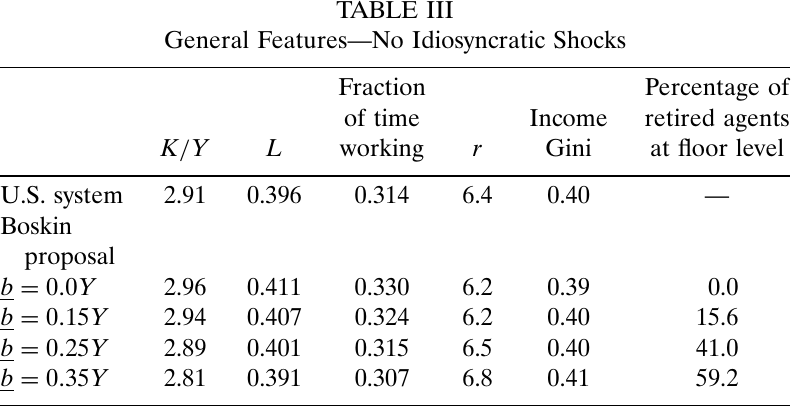
\includegraphics[width=130mm]{./OriginalTablesFigures/HV1999_Table3.png}\\[6mm]
\input{../SavedOutput/LatexInputs/HV1999_Table3.tex}
\end{tabular}
\end{center}
\caption{Table III of Huggett \& Ventura (1999): general features, no idiosyncratic shocks.
Top: original from paper. Bottom: replicated.}
\label{tab:table3}
\end{table}

\begin{table}[htp]
\begin{center}
\begin{tabular}{c}
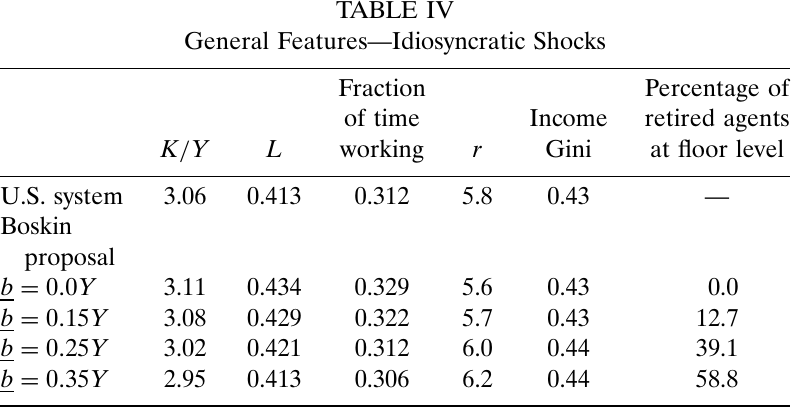
\includegraphics[width=130mm]{./OriginalTablesFigures/HV1999_Table4.png}\\[6mm]
\input{../SavedOutput/LatexInputs/HV1999_Table4.tex}
\end{tabular}
\end{center}
\caption{Table IV of Huggett \& Ventura (1999): general features, idiosyncratic shocks.
Top: original from paper. Bottom: replicated.}
\label{tab:table4}
\end{table}

\begin{table}[htp]
\begin{center}
\begin{tabular}{c}
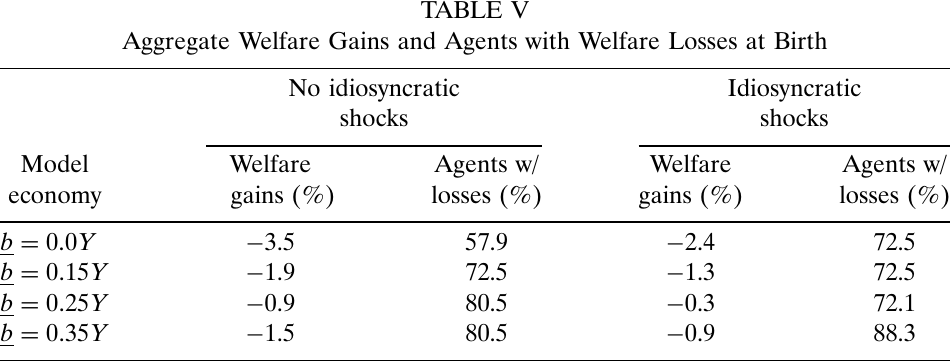
\includegraphics[width=130mm]{./OriginalTablesFigures/HV1999_Table5.png}\\[6mm]
\input{../SavedOutput/LatexInputs/HV1999_Table5.tex}
\end{tabular}
\end{center}
\caption{Table V of Huggett \& Ventura (1999): aggregate welfare gains and agents with welfare
losses at birth, under the Boskin proposal. Top: original from paper. Bottom: replicated.}
\label{tab:table5}
\end{table}

\begin{table}[htp]
\begin{center}
\begin{tabular}{c}
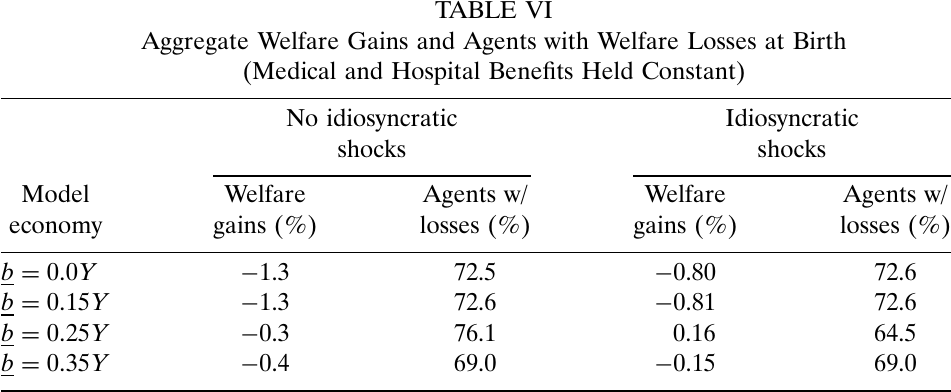
\includegraphics[width=130mm]{./OriginalTablesFigures/HV1999_Table6.png}\\[6mm]
\input{../SavedOutput/LatexInputs/HV1999_Table6.tex}
\end{tabular}
\end{center}
\caption{Table VI of Huggett \& Ventura (1999): the same welfare measures with the medical and
hospital transfer held constant across systems. Top: original from paper. Bottom: replicated.}
\label{tab:table6}
\end{table}

% ----------------------------------------------------------------- Figures
\begin{figure}[htp]
\begin{center}
\begin{tabular}{c}
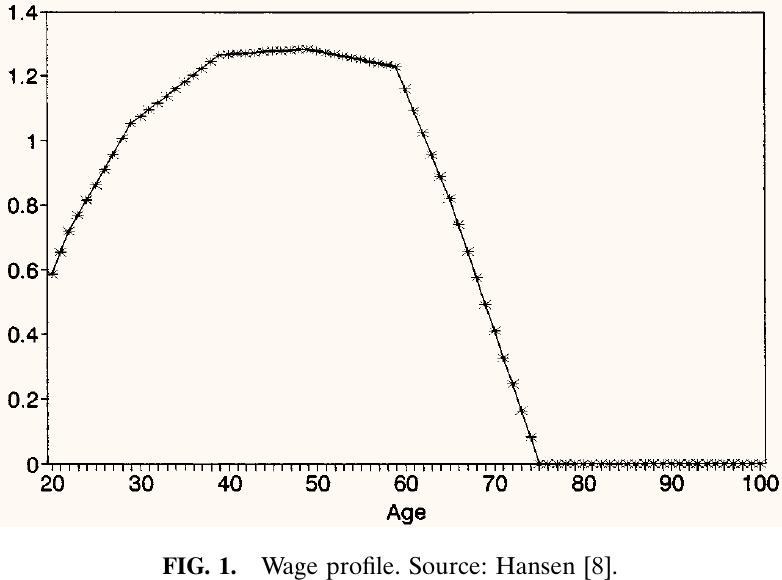
\includegraphics[width=95mm]{./OriginalTablesFigures/HV1999_Fig1.png}\\[4mm]
\includegraphics[width=120mm]{../SavedOutput/Graphs/HV1999_Fig1_WageProfile.png}
\end{tabular}
\end{center}
\caption{Figure 1 of Huggett \& Ventura (1999): the age-efficiency profile. Top: original from
paper. Bottom: replicated, with Hansen's tabulated age-group values shown as markers.}
\label{fig:fig1}
\end{figure}

\begin{figure}[htp]
\begin{center}
\begin{tabular}{c}
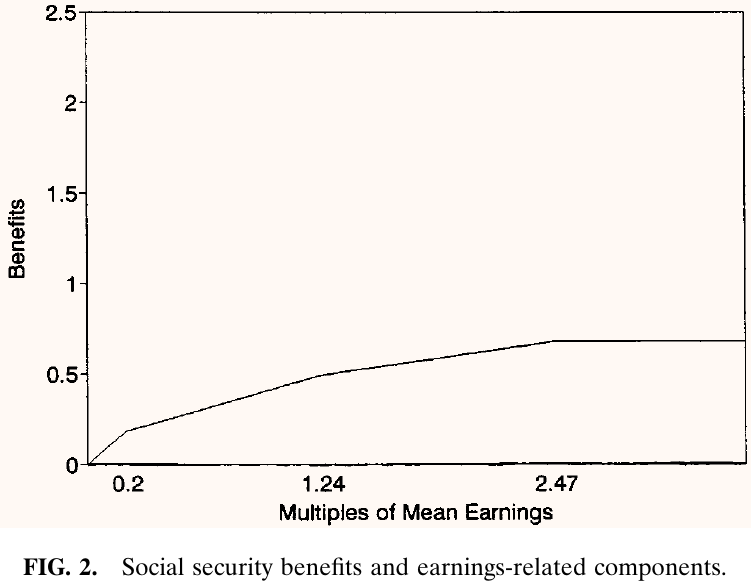
\includegraphics[width=95mm]{./OriginalTablesFigures/HV1999_Fig2.png}\\[4mm]
\includegraphics[width=120mm]{../SavedOutput/Graphs/HV1999_Fig2_Benefits_noidio.png}
\end{tabular}
\end{center}
\caption{Figure 2 of Huggett \& Ventura (1999): social security benefits as a function of
average past earnings. Top: original from paper. Bottom: replicated, showing the total
benefit, the concave earnings-related component, and the common medical transfer separately.
The kinks are the bend points at $0.20$ and $1.24$.}
\label{fig:fig2}
\end{figure}

\begin{figure}[htp]
\begin{center}
\begin{tabular}{c}
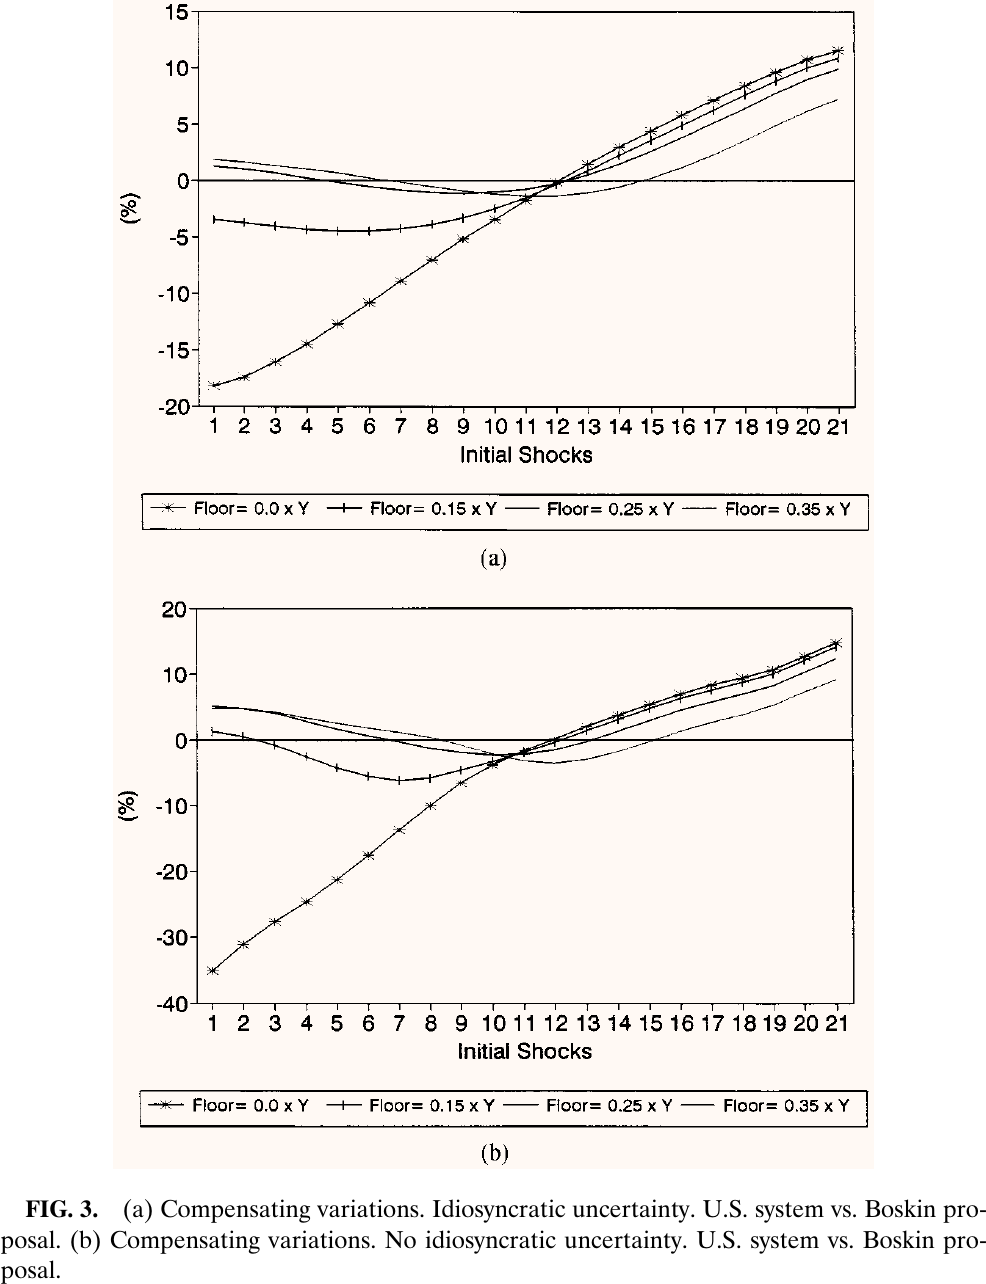
\includegraphics[width=88mm]{./OriginalTablesFigures/HV1999_Fig3.png}\\[4mm]
\includegraphics[width=150mm]{../SavedOutput/Graphs/HV1999_Fig3_CEV.png}
\end{tabular}
\end{center}
\caption{Figure 3 of Huggett \& Ventura (1999): compensating variations, U.S.\ system versus
Boskin proposal, by ability at birth. Top: original from paper, panel (a) with idiosyncratic
uncertainty and panel (b) without. Bottom: replicated, same panel ordering.}
\label{fig:fig3}
\end{figure}

\begin{figure}[htp]
\begin{center}
\begin{tabular}{c}
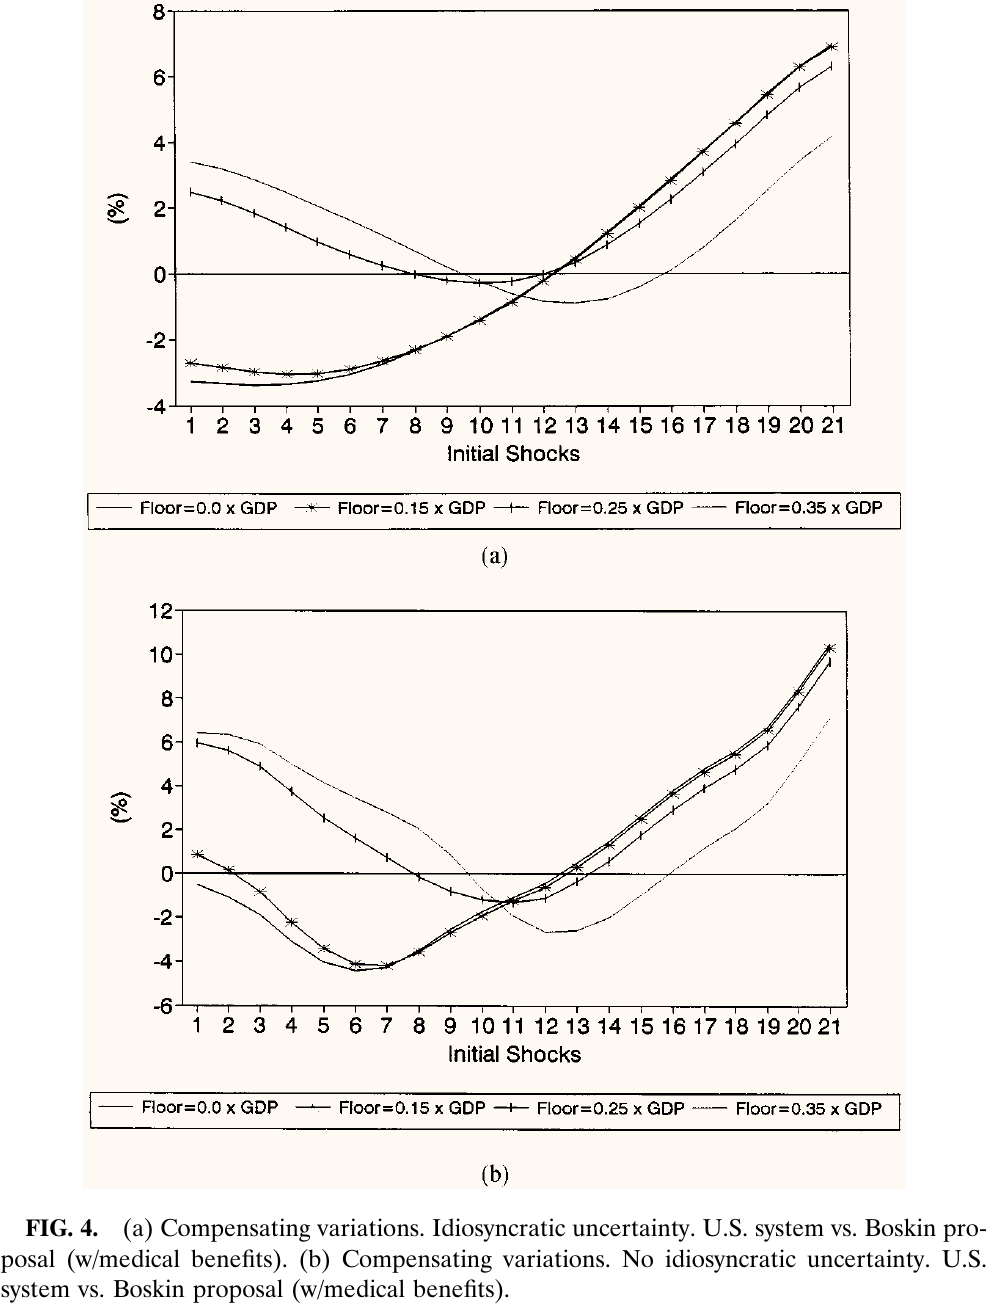
\includegraphics[width=88mm]{./OriginalTablesFigures/HV1999_Fig4.png}\\[4mm]
\includegraphics[width=150mm]{../SavedOutput/Graphs/HV1999_Fig4_CEV.png}
\end{tabular}
\end{center}
\caption{Figure 4 of Huggett \& Ventura (1999): compensating variations with the medical and
hospital transfer retained in both systems. Top: original from paper. Bottom: replicated.}
\label{fig:fig4}
\end{figure}

\begin{figure}[htp]
\begin{center}
\begin{tabular}{c}
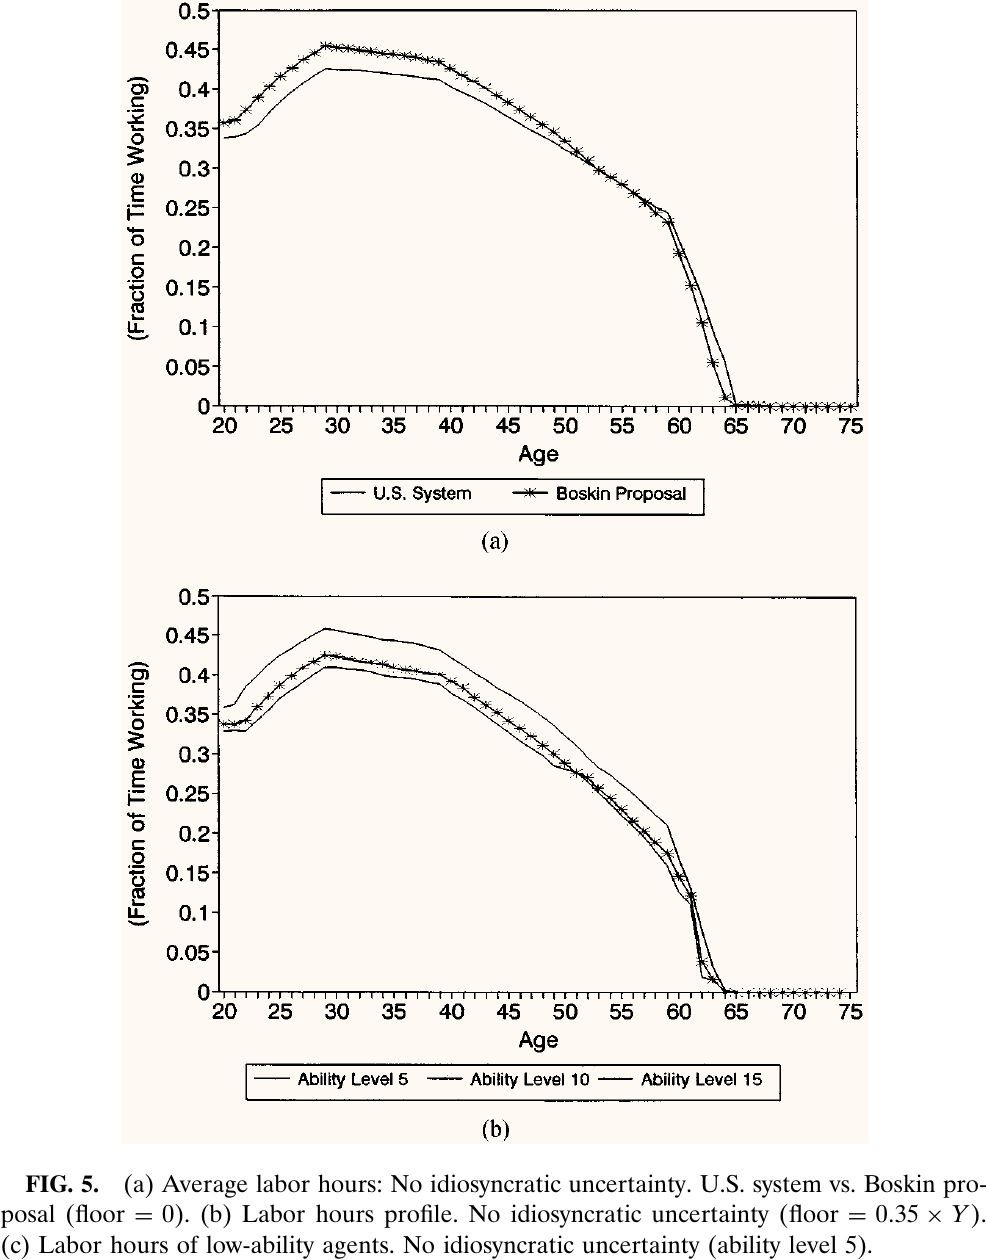
\includegraphics[width=86mm]{./OriginalTablesFigures/HV1999_Fig5.png}\\[2mm]
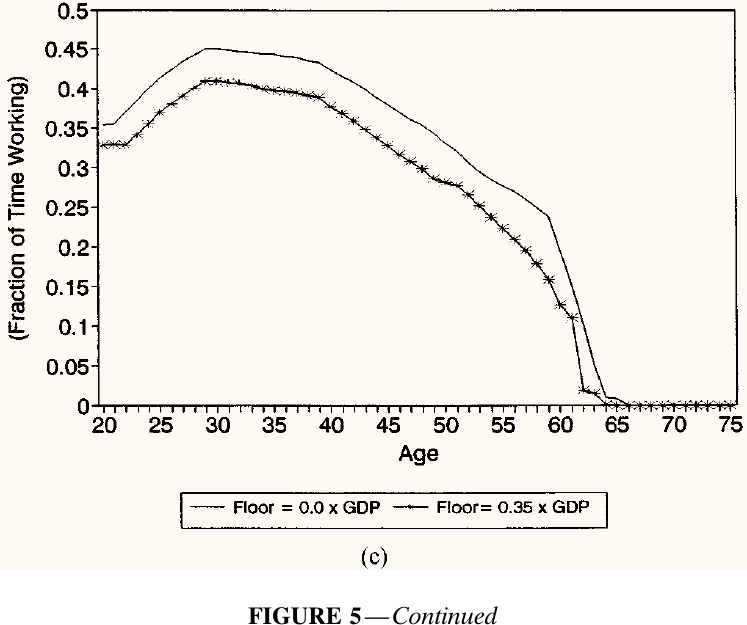
\includegraphics[width=86mm]{./OriginalTablesFigures/HV1999_Fig5c.png}\\[4mm]
\includegraphics[width=160mm]{../SavedOutput/Graphs/HV1999_Fig5_Hours.png}
\end{tabular}
\end{center}
\caption{Figure 5 of Huggett \& Ventura (1999): average labour hours over the life cycle, no
idiosyncratic uncertainty. Top: original from paper, panels (a) and (b) then the continued panel (c).
Bottom: replicated. Panel (c), the low-ability agent, carries the mechanism: a zero floor raises hours above the U.S.\ system,
while a floor of $0.35Y$ lowers them from about age 40.}
\label{fig:fig5}
\end{figure}

\begin{figure}[htp]
\begin{center}
\begin{tabular}{c}
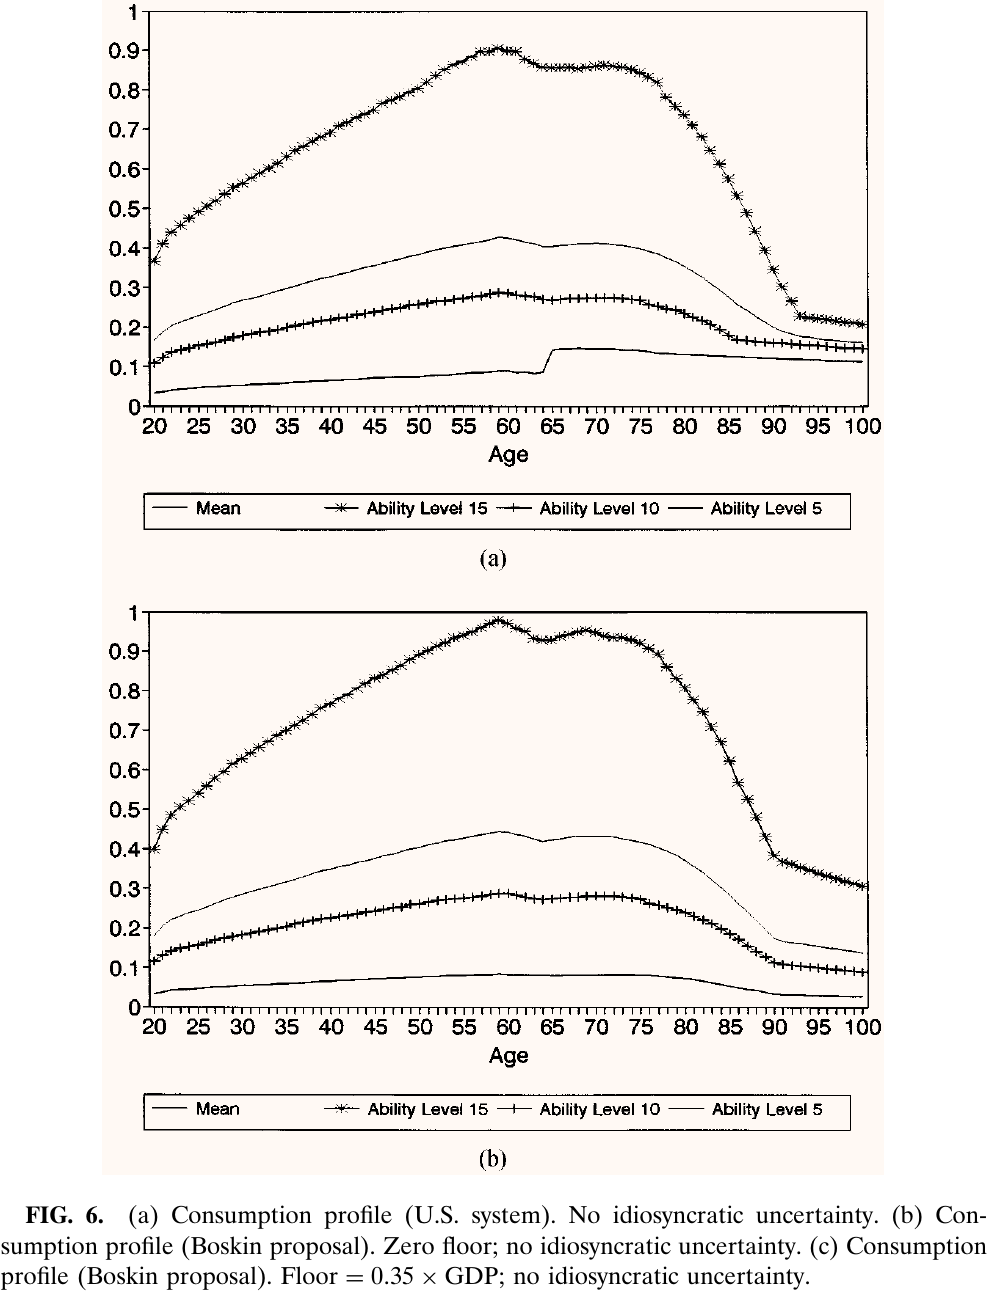
\includegraphics[width=86mm]{./OriginalTablesFigures/HV1999_Fig6.png}\\[2mm]
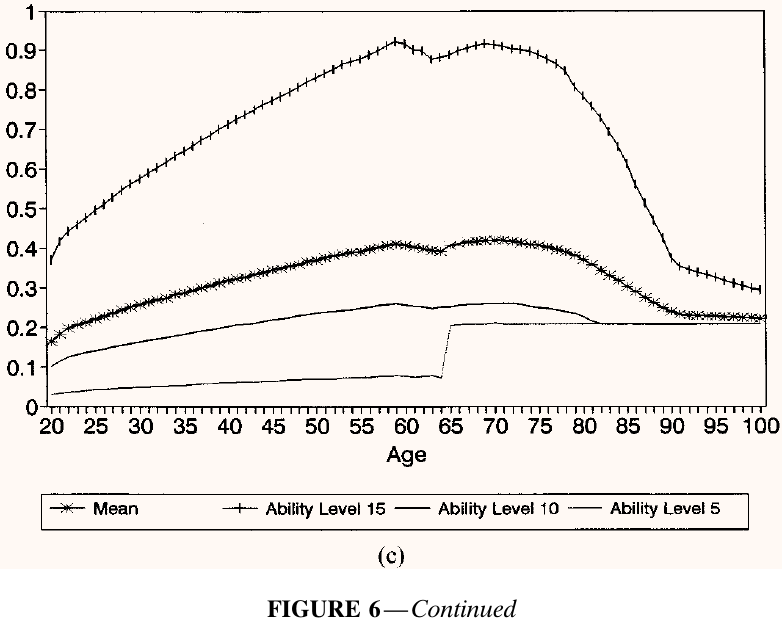
\includegraphics[width=86mm]{./OriginalTablesFigures/HV1999_Fig6c.png}\\[4mm]
\includegraphics[width=160mm]{../SavedOutput/Graphs/HV1999_Fig6_Consumption.png}
\end{tabular}
\end{center}
\caption{Figure 6 of Huggett \& Ventura (1999): consumption profiles, no idiosyncratic
uncertainty. Top: original from paper, panels (a) and (b) then the continued panel (c).
Bottom: replicated; the heavy line is the population average and the light lines are ability
levels 5, 10 and 15, the three the paper's own legend names.}
\label{fig:fig6}
\end{figure}


\clearpage

\appendix
\section{Computational details}\label{sec:computational}

\paragraph{State space.} The U.S.\ system has endogenous states $(a,\bar{e})$ on a
$251\times 25$ grid and the Boskin systems $(a_1,a_2)$ on $251\times 50$. The asset grid uses
the paper's own curvature, $a_k = \bar{a}(k/K)^{2.35}$, with $\bar{a}=40$; the private asset
grid is identical across systems, because the compensating variations compare the two steady
states at the same newborn state. HV1999 uses $101$ points on assets, $4$ on $\bar{e}$ and
$21$ on $z$; we keep $21$ on $z$ (footnote 17) but refine the endogenous grids, because four
points cannot carry an accumulating average. The labour choice is discretized at 75 points,
where the paper uses golden-section search; moving between $51$ and $101$ points changes every
aggregate by less than one part in $10^{4}$, and leaves the compensating variations unchanged
at the printed precision.

\paragraph{The $a_2$ ceiling.} Accumulated contributions are bounded above in this model
rather than merely unlikely to be large: the productivity grid tops out at
$\exp(4\sigma_{y_1})$, so even an agent drawing the highest shock every year and working
$l=1$ every year reaches only $a_2=98.0$ at the equilibrium prices of the idiosyncratic
economy. The ceiling is sensitive to $r$ through 45 years of compounding at $(1+r)/(1+g)$ ---
$79.6$ at $r=5\%$, $133.0$ at $r=7\%$ --- so the grid is taken to $150$, which cannot bind for
any interest rate below about $7.3\%$. Diagnostics confirm it: the mass in the top ten $a_2$
grid points is $7.6\times10^{-10}$.

\paragraph{Grid-top diagnostics.} Every stage reports the mass sitting in the top grid points
of each endogenous state. The $a_2$ ceiling is never approached. The asset ceiling
$\bar{a}=40$ carries $1.7\times10^{-4}$ of the mass in its top ten points under the
idiosyncratic U.S.\ system, slightly above our $10^{-5}$ reporting threshold; widening it
moves an income Gini that currently matches the paper exactly, so it is reported rather than
tuned away.

\paragraph{Solution method.} Value function iteration with divide-and-conquer and a
grid-interpolation layer on the asset dimension. General equilibrium is solved by Anderson
acceleration of the shooting map, which converges in eight to ten iterations from a warm start
at every floor level. Successive floor levels are solved in increasing order, each starting
from the previous level's equilibrium.

\paragraph{Reproducing these results.} The driver is \texttt{HuggettVentura1999.m}, with the
wage specification selected by \texttt{idioShocks} and the work split into seven stages by the
\texttt{doPart} vector: the U.S.\ steady state; the Boskin proposal at each floor level; the
compensating variations; the medical-benefits variant at each floor level; its compensating
variations; the age profiles; and the figures. The floor levels solved in a given job are
selected by \texttt{doFloorsB} and \texttt{doFloorsM}, so a single level can be re-run on its
own, and each level writes its own \texttt{.mat}. Tables III--VI are assembled in the final
stage from those files, so levels solved in different jobs combine.

\end{document}
